\chapter{Testing and Evaluation}
\label{chapter:testing-and-eval}
The purpose of this chapter is to evaluate how effective the developed mobile application is in respect to applying the behaviour change theory discussed in Chapter \ref{Chapter:Literature-Review}. To examine this, a series of tests were performed, namely: \textit{Acceptance}, \textit{Functional} and \textit{Usability} testing. Furthermore, a survey was carried out with three university students in order to obtain general user opinion regarding varying aspects of the application. The tests performed on the system are going to be discussed first followed by a discussion on how the system compares with a current commercial product in the same field. Finality, the survey responses are examined.

\section{Acceptance Testing}
Acceptance testing is a key part of the software development process. It evaluates weather the software conforms with the client requirements. Consequently, it is determined if the end-product is capable of performing the specified functionality. The following sub-components of the system underwent Acceptance testing, namely: \textit{Goal-Setting Component} (\gls{gsc}), \textit{Monitoring Component} (\gls{mc}) and \textit{Feedback Component} (\gls{fc}).

\subsection{Goal-Setting Component}
The three specifications for this component were all implemented successfully. The list of the implemented requirements can be seen in Table \ref{tab:gsc-acceptance-tests}. 

\begin{itemize}
    \item \textit{"\gls{gsc} shall provide list of recommended \gls{pa} goals"} - is implemented by utilising an Android framework component called \textit{Dialog} \citep{androiddialogs_2017}. A Dialog window is presented to the user so they can choose their \gls{pa} goal in minutes (e.g. 10, 20, 30, 60).
    \item \textit{"\gls{gsc} shall automatically set the recommended \gls{pa} goal if the user does not explicitly do so"} is implemented in the \textit{initial setup} set of screens discussed in section \ref{section:initial-setup-screens}. If the user decides to skip the \textit{initial-setup} screens (which offer options such as setting the \gls{pa}, \gls{mci} and the \textit{Sleeping Hours} time interval) default values are set. For example, the \gls{pa} goal is set to 30 minutes, \gls{mci} (or the \gls{st} goal) is set to 60 minutes and the \textit{Sleeping Hours} time interval is set to 8pm to 8am. 
    \item \textit{"\gls{gsc} shall allow the user to set a Maximum Continuous Inactivity (MCI)..."} is successfully implemented using a dialog window. It allows the user to set their \gls{st} (or \gls{mci}) goal by selecting it from a list of preset values in the dialog. In addition to the \textit{initial setup} screens the user is able to do that in the \textit{Settings} screen. 
\end{itemize}
 

\begin{table}[ht]
    \centering
    \tabulinesep=1.5mm
  \begin{longtabu} to \textwidth {|X|c|X|}
    \hline
      \textbf{Specification}
      & \textbf{Status}
      & \textbf{Notes}
    \endhead \hline
    \gls{gsc} shall provide list of recommended \gls{pa} goals
      & Implemented
      & 
    \\ \hline
    \gls{gsc} shall automatically set the recommended \gls{pa} goal if the user does not explicitly do that 
    & Implemented
    & If the user does not set a goal during the initial-setup, the app sets the recommended daily activity levels
    \\ \hline
    \gls{gsc} shall allow the user to set a Maximum Continuous Inactivity (MCI) before a reminding notification is sent 
    & Implemented
    & 
    \\ \hline
 \end{longtabu}
    \caption{\gls{gsc} acceptance tests}
    \label{tab:gsc-acceptance-tests}
\end{table}




\subsection{Monitoring component}
Four out of the five initially set features were fully implemented. The list of the implemented requirements can be seen in Table \ref{tab:mc-acceptance-tests}. First of those features - \textit{HAR component shall recognise 4 activities(walking, running, cycling and static)} was implemented by gathering activity data from fellow university students and training a classifier to recognise the above-mentioned activities.


\begin{table}[ht]
    \centering
    \tabulinesep=1.5mm
  \begin{longtabu} to \textwidth {|X|c|X|}
    \hline
      \textbf{Specification}
      & \textbf{Status}
      & \textbf{Notes}
    \endhead \hline
    \gls{mc} component shall classify four physical activities
    & Implemented
    & The classifier is trained to recognise \textit{walking}, \textit{running}, \textit{cycling} and \textit{static}
    \\ \hline
    \gls{mc} shall the increment user's \gls{pa} or \gls{st} value whenever physical activity or sedentary behaviour is recognised
    & Implemented
    & 
    \\ \hline
    The \gls{mc} shall personalise \gls{har}'s classifier
    & Not implemented
    & Due to the time constraints of the project this feature was not implemented.
    \\ \hline
    The system shall allow the user to group the collected data in "Daily" and "Weekly" representation
    & Implemented
    & This is implemented in the History screen of the application
    \\ \hline
    The user shall be able to set the \textit{Sleeping Hours Time Interval} (\gls{shti}) during which no measurement of \gls{pa} or \gls{st} should occur
    & Implemented
    & 
    \\ \hline
 \end{longtabu}
    \caption{\gls{mc} acceptance tests}
    \label{tab:mc-acceptance-tests}
\end{table}


As far as \textit{\gls{mc} shall increment user's \gls{pa} or \gls{st} value whenever physical activity or sedentary behaviour is recognised} is concerned, this feature was implemented in the \textit{ActivityMonitor} class (see section \ref{section:activity-monitor}). This class is responsible for incrementing the activity and inactivity values depending on the recognised class by the classifier.

\textit{The system shall allow the user to group the collected data in "Daily" and "Weekly" representation}. This feature was implemented in the \textit{History} screen of \textit{ActiveMinutes}. The \gls{ui} of this screen includes \textit{DAILY} and \textit{WEEKLY} buttons allowing the user to switch between both representations of the collected data, accordingly.

The next requirement - \textit{The user shall be able to set the \textit{Sleeping Hours} time interval during which no measurement of \gls{pa} or \gls{st} should occur} - was implemented in the \textit{Settings} screen. The \gls{ui} of this screen provides the user with the option to change their \textit{Sleeping Hours} time interval by tapping on the appropriate menu item and choosing the desirable start and end times.

There were some features of the system that were not implemented since it was determined to be too complex given the project time constraints. One of those feature was \textit{The \gls{mc} shall personalise \gls{har}'s classifier}. This feature was discussed in section \ref{section:classifier-personal-service} and it has been designed as Android \textit{Service}. It uses the gathered-with-time and filtered by the classifier's confidence level data (e.g. above 80\% - to filter only the recognised activities with high confidence). The service combines this data with the general one and produces a personalised model that is used for further classification. According to \citet[376]{arapakis_athanasakos_jose_2010}, that is expected to improve the classifier's accuracy.


\subsection{Feedback Component}
As far as the \gls{fc} is concerned, a total of three features were successfully implemented (see Table \ref{tab:fc-acceptance-tests}. One of the initial requirements of the \gls{fc} was not implement due to the project's time constrains. \textit{FeedbackProvider} (see section \ref{section:feedback-provider}) represents the \gls{fc} implementation system-wise. The first requirement - \textit{\gls{fc} shall notify the user when they are being sedentary for 1 hour} allows the user to be notified for a prolonged sedentary time. This feature was implemented by utilising Android's \textit{Notification} API. In addition, this API is used to satisfy another feature as well, namely \textit{\gls{fc} shall notify the user when a previously set goal is attained}. It allows the user to be notified when they achieve their daily goal (e.g. 30 minutes of \gls{pa}).

\begin{table}[ht]
    \centering
    \tabulinesep=1.5mm
  \begin{longtabu} to \textwidth {|X|c|X|}
    \hline
      \textbf{Specification}
      & \textbf{Status}
      & \textbf{Notes}
    \endhead \hline
    \gls{fc} shall notify the user when they are being sedentary for 1 hour (or the value set by the user) as recommended by \citet[]{swartz2011}
    & Implemented
    & 
    \\ \hline
    \gls{fc} shall notify the user when a previously set goal is attained (e.g. being active for 30 minutes)
    & Implemented
    & 
    \\ \hline
    \gls{fc} shall not send notifications during the "Sleeping Hours" time interval
    & Implemented
    & 
    \\ \hline
    \gls{fc} shall send a notification to the user every Sunday to show goal-performance feedback for the past week
    & Not Implemented
    & Although good to have, due to time constraints this feature was not implemented.
    \\ \hline
 \end{longtabu}
    \caption{\gls{fc} acceptance tests}
    \label{tab:fc-acceptance-tests}
\end{table}

Another feature implemented feature - \textit{\gls{fc} shall not send notifications during the user set "Sleeping Hours" time interval} makes sure that the system stops monitoring user's \gls{pa} and \gls{st} levels when \textit{Sleeping Hours} time interval is entered. 

Last but not least, \textit{\gls{fc} shall send a notification to the user every Sunday to show goal-performance feedback for the past week} - a feature (or rather a screen) which provides more information to the user regarding their goal-performance in comparison the only receiving notifications. Although "good-to-have", this feature was not implemented due to the project's time constrains rather than lack of technical capability.

\section{Functional Testing}
This is quality assurance (QA) testing that aims to verify that the system is providing the same output as required by the end user. Each test has an input, expected result, actual result and states whether the system passes the test or not.

Every feature of the system was tested to ensure that it works and satisfies the functional requirements of the system. For example, test cases verified that if the navigation of the system works as expected, e.g.\ when the user presses the \textit{History} menu item of the navigational drawer, that takes the user to this screen. Also, self-management was tested as well, e.g.\ the goal-setting, monitoring and feedback components. For example, to test the monitoring component of the system the user (one of the project participants) had to perform 5 minutes of \gls{pa} or \gls{sb}. The result was compared with the \textit{Actual result} (if the system measures successfully the above amount). A snippet of the monitoring component functional testing can be seen in Table \ref{tab:monitoring-com-ft}.

\begin{table}[ht]
    \centering
    \fontsize{9}{12}\selectfont
    \tabulinesep=1mm
  \begin{longtabu} to \textwidth {|l|X|X|X|l|l|}
    \hline
      \textbf{Step No}
      & \textbf{Test Cases}
      & \textbf{Expected result}
      & \textbf{Actual result}
      & \textbf{Status}
    \endhead \hline
    1
    & \raggedright The user starts the mobile application and performs 5 minutes of \textbf{walking}.
    & \raggedright The system should recognise that the user is performing \gls{pa} and increments \textit{Active} time. 
    & \raggedright Works as expected e.g., updates the \gls{ui} by adding 5 minutes to the \gls{pa} progress bar in \textit{Today} \& \textit{History} screens.
    & Pass
    \\ \hline
    2
    & \raggedright The user starts the mobile application and performs 5 minutes of \textbf{running}.
    & \raggedright The system should recognise that the user is performing \gls{pa} and increments \textit{Active} time. 
    & \raggedright Works as expected e.g., updates the \gls{ui} by adding 5 minutes to the \gls{pa} progress bar in \textit{Today} \& \textit{History} screens.
    & Pass
    \\ \hline
\end{longtabu}
    \caption{Monitoring activity functional test snippet}
    \label{tab:monitoring-com-ft}
\end{table}

A total of 30 test cases in different categories were created to ensure that every implemented feature of the system is tested. The system successfully passes all of the tests. The device used during the tests was \textit{Google Pixel} \footnote{\url{https://madeby.google.com/intl/en_uk/phone/}}. All test cases can be seen in Appendix \ref{chapter:functional-testing}.

\section{Usability Testing}
In addition to acceptance and functional testing, usability testing has been performed on the system to determine if it is easy to use. The usability test consisting of 16 tasks that the real user (i.e., one of the project participants) performed on the system. Two of the tests can be seen in Table \ref{tab:usability-test-snippet}. The full list of the tasks can be seen in Appendix \ref{chapter:usability-testing}.

\begin{table}[ht]
    \centering
    \fontsize{9}{12}\selectfont
    \tabulinesep=1mm
  \begin{longtabu} to \textwidth {|l|X|X|l|}
    \hline
      \textbf{Task No}
      & \textbf{Task}
      & \textbf{Comments}
      & \textbf{Status}
    \endhead \hline
    1
    & \raggedright Open the application and create an account.
    & \raggedright The user was able to understand what was required and complete the process by accessing the Sign-up screen, entering their credentials and selecting the \textit{SIGN UP} button.
    & Pass
    \\ \hline
    2
    & \raggedright Navigate to the \textit{Today} screen and describe what you are seeing.
    & \raggedright The user was able to explain correctly the purpose of the screen i.e., the screen shows the current activity and inactivity goals as well as their progress
    & Pass
    \\ \hline
\end{longtabu}
    \caption{Usability test snippet}
    \label{tab:usability-test-snippet}
\end{table}

The results from the test indicate that the user finds the mobile application easy to use. For example the user was able to understand how to perform all of tasks part of the test. However, when asked to explain the functionality \textit{History} screen, the user spend more time trying to make the connection between the top \gls{pa} and \gls{mci} labels and the two progress bars. This confusion can be easily fixed by adding a text label above each of the progress bars to indicated which is one is displaying \gls{pa} and \gls{mci}.

All of the usability tests indicate that the mobile application is fairly easy to understand and use. The user was able to complete all tests successfully. It is worth mentioning that the user was familiar with the Android platform prior to the test. That means that standard icons such as the icon used to indicate the presents of a navigational drawer was already familiar to the user which made the task of accessing the different screens of the application a lot easier. Future usability tests should include a wider range of users.
\newpage
\section{Comparing the system with commercial solutions}
The system has been compared with a commercial mobile application currently available in the market, namely \textit{Human}\footnote{\url{http://human.co}} that offers similar functionality. The two systems have been compared regarding battery consumption, classifier technology used and the main features each of the systems offers. To do the comparison, the two applications have been installed on \textit{Google Pixel} device and evaluated for a full day. The following subsections will discuss the evaluation findings.

\subsection{Battery consumption}
The battery consumption of both application has been evaluated by using an Android an android application called \textit{AccuBattery}\footnote{\url{https://play.google.com/store/apps/details?id=com.digibites.accubattery&hl=en_GB}}. The results show that \textit{ActiveMinutes} uses a considerable amount of battery in comparison to \textit{Human}. According to the \textit{AccuBattery} measurements, \textit{ActiveMinutes} consumed about 150 mAh for the duration of the one day evaluation. That is a lot more then what \textit{Human} consumed - 34 mAh.

\subsection{Classifier technology}
As it was discussed in section \ref{section:classifier}, \textit{ActiveMinutes} trains a classifier online whereas \textit{Human} uses \textit{Google Fit} to perform the monitoring of the user offline. Building a classifier online introduces several advantages. Firstly, \textit{ActiveMinutes}'s classifier can be personalised since it is built online. Secondly, the application can work completely offline, meaning that \textit{ActiveMinutes} does not require an Internet connection to function. 

Having said that, \textit{ActiveMinutes} has several disadvantages. Since \textit{Human} uses \textit{Google Fit} to perform the monitoring, it uses a combination of sensors such as GPS to perform \gls{har}. That means that the system is less likely to recognise involuntary movements of the device as \gls{pa}. For example, if the user is sitting on a couch and moving their smartphone up and down, the system would not recognise that as \gls{pa}. Although, \textit{ActiveMinutes} keeps track of the last three activities to minimise the classification of these involuntary movements as \gls{pa} it is easy to "fool" the system by going through the above-mentioned example.

\subsection{Features}
Feature-wise, \textit{ActiveMinutes} offers a wider range of goals the user can set in comparison to what \textit{Human} offers. For example, 10, 20, 30, 60, 120 and 30, 60 and 90 minutes are the possible values the user can choose from when setting \gls{pa} and \gls{sb} goals, respectively. For comparison, \textit{Human} offers only three values for both \gls{pa} and \gls{sb} goals: 30, 60 an 120 (see figure \ref{figure:comparison-with-human}). By offering a wider range of goal values the user can make a smoother transition from doing 10 minutes of physical activity per day to doing up to 2 hours. In addition to providing a winder range of goal values, \textit{ActiveMinutes} offers the user the option to change their \textit{SleepingHours} interval ("Inactivity nudge" in \textit{Human}) whereas this value in \textit{Human} is pre-set i.e. 9AM - 7PM.

\begin{figure*}[ht]
    \centering
    \begin{subfigure}[t]{0.4\textwidth}
        \centering
        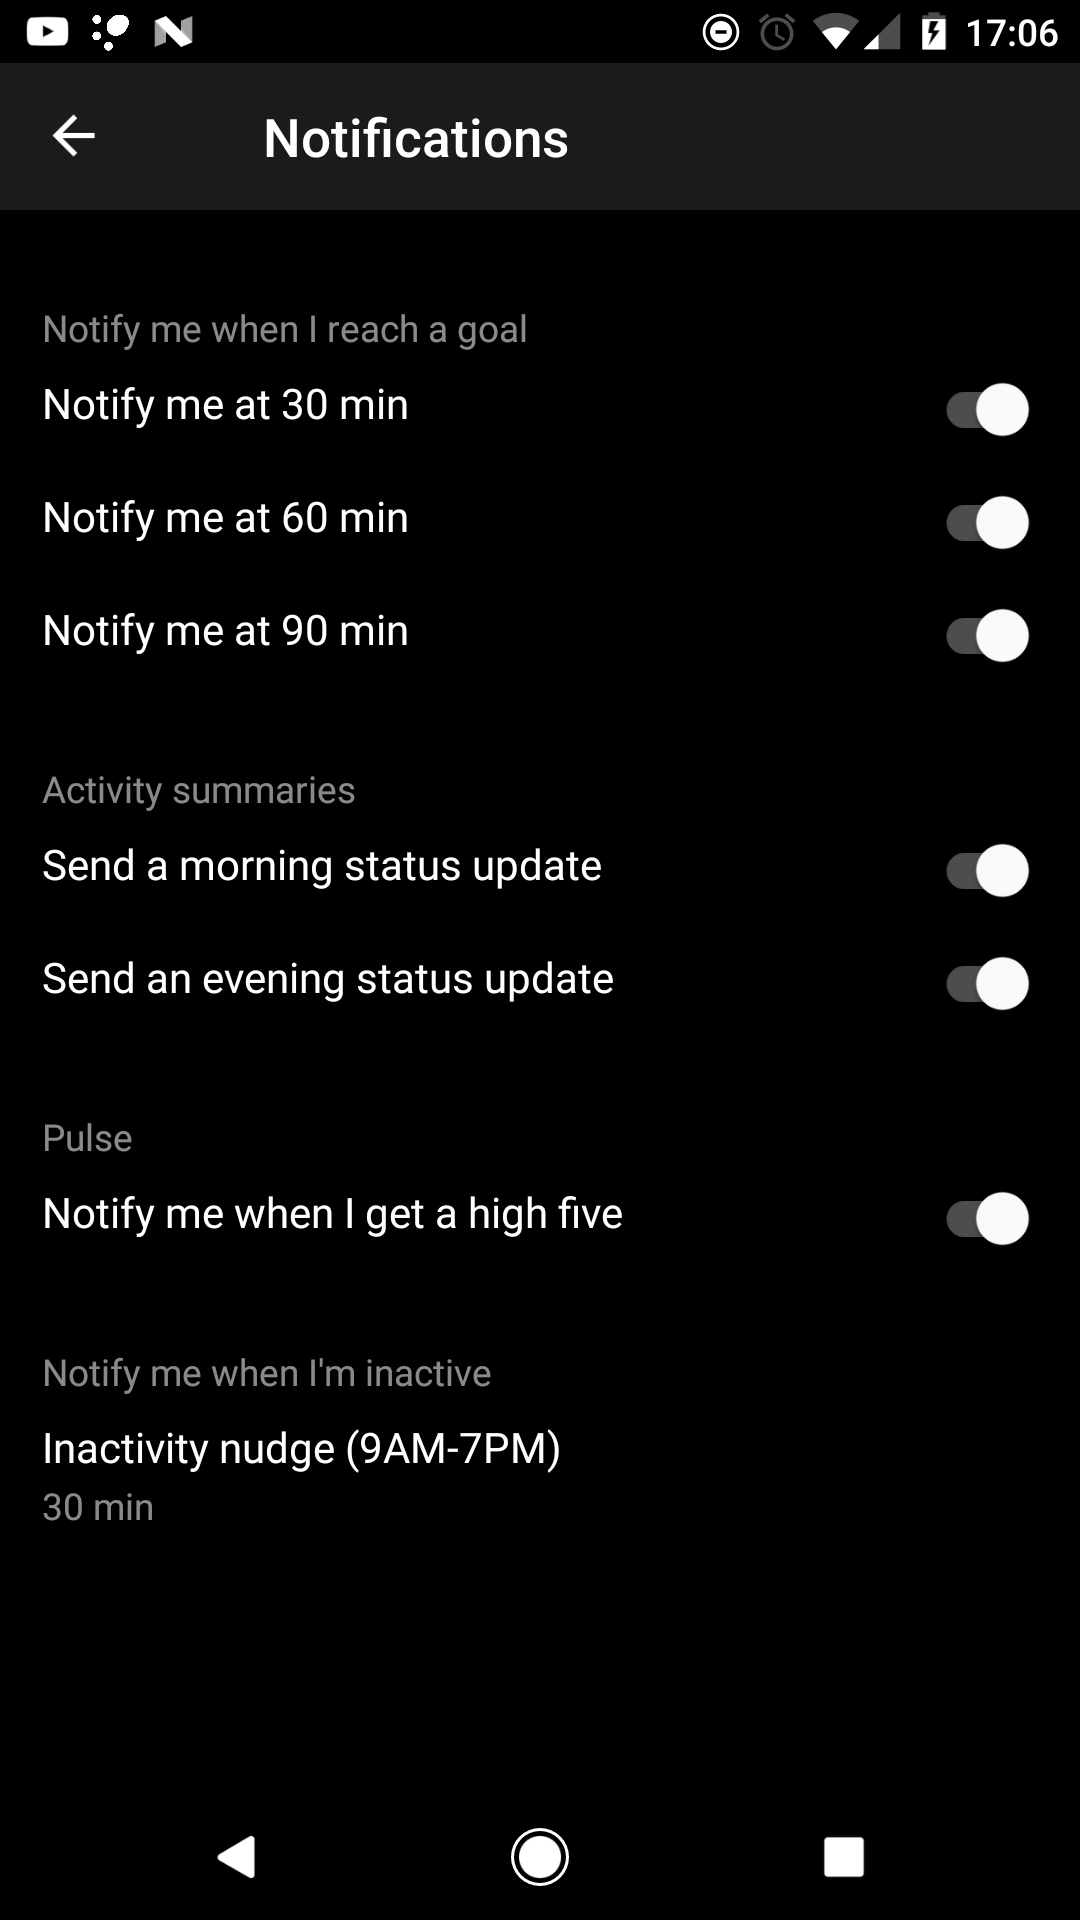
\includegraphics[width=3cm,keepaspectratio]{human_settings_screenshot}
        \caption{\textit{Human}}
    \end{subfigure}%
    ~ 
    \begin{subfigure}[t]{0.4\textwidth}
        \centering
        \frame{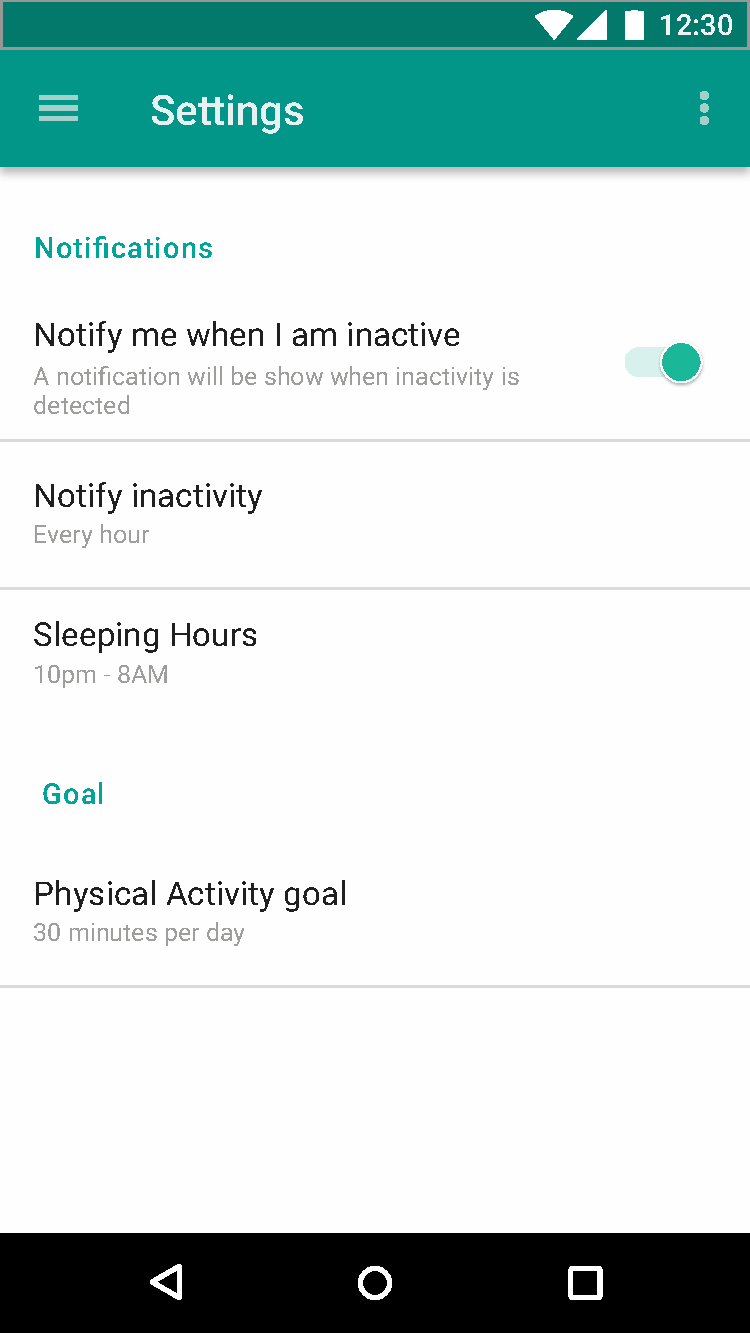
\includegraphics[width=3cm,keepaspectratio]{settings-screen-design}}
        \caption{\textit{ActiveMinutes}}
    \end{subfigure}
    \caption{Comparing the system with other solutions}
    \label{figure:comparison-with-human}
\end{figure*}

Having said that, \textit{Human} offers several features which are not present in \textit{ActiveMinutes}. For example, the user can compare their goal-performance with the performance of nearby people who are using the app as well. Also, \textit{Human} shows a breakdown of the \gls{pa}. For example, the user can see how much time they spend walking or cycling. 

\section{Survey results}
In order to test \textit{ActiveMinutes}'s performance in a real-life scenario, the mobile application was installed on a total three university students mobile phones. It was used for an entire day before the participants had to share their feedback via a survey. A survey contained a total of 9 questions, a snippet of the survey can be seen in Table \ref{tab:user-survey-extract}. Each survey question and summary response are going to be discussed next. All questions can be seen in Appendix \ref{chapter:survey-results}.

\begin{table}[ht]
    \centering
    \ \fontsize{9}{12}\selectfont
\tabulinesep=.5mm
\begin{longtabu} to \textwidth {|l|l|l|}
\hline
    No
    & \textbf{Question}
    & \textbf{Response summary}
    \endhead \hline
    1
    & \makecell[l]{Were you more active then usual (e.g. walking, running)\\ as a result of using ActiveMinutes?}
    & \makecell[l]{Yes (33.33\%)\\ No (33.33\%)\\  Not sure (33.33\%)}
    \\ \hline
    2
    & \makecell[l]{When notified for prolonged inactivity (e.g. 30 minutes of inactivity),\\ did you try to do at least 5 minutes of physical activity?}
    &\makecell[l]{Yes (66.67\%)\\ No (0\%)\\  Sometimes (33.33\%)}
    \\ \hline
    3
    & \makecell[l]{Do you think the application was accurate when measuring your\\ activity levels?}
    & \makecell[l]{Yes (66.67\%)\\ No (0\%)\\  Somewhat (33.33\%)}
    \\ \hline
    4
    & \makecell[l]{How easy to understand was the user interface of the application?\\ (0 being very difficult and 100 being very easy)}
    & \makecell[l]{Response 1 - 100\\ Response 2 - 80\\ Response 3 - 75\\ \textbf{Average - 85}}
    \\ \hline
\end{longtabu}
    \caption{User survey extract}
    \label{tab:user-survey-extract}
\end{table}

\begin{itemize}
    \item \textit{What is your age?}
    According to the survey, all of the participant's age was between 18 and 24 years. Future evaluations of the system may consider including different age groups to find out how the system works for them.
    \item \textit{Were you more active then usual (e.g. walking, running) as a result of using ActiveMinutes?}
    In general, the mobile application had a positive impact on two of the project participants. However, the third participant did not see any improvement in their level of \gls{pa}. 
    \item \textit{When notified for prolonged inactivity (e.g. 30 minutes of inactivity), did you try to do at least 5 minutes of physical activity?}
    Overall, the mobile application had a positive effect on the project participants. Two people responded "Yes" and only one responded "Sometimes". 
    \item \textit{Does seeing past days goal-performance (e.g. in the History screen) motivate you to achieve a goal?}
    All of the survey participants answered "Yes" to this question.
    \item \textit{Does the visual feedback (i.e. the green progress bar) encourage you to achieve your goal?}
    All of the survey participants answered "Yes" to this question.
    \item \textit{Do you think the application was accurate when measuring your activity levels?}
    Two of the three survey participants responded "Yes" to this question where as the other participant answered "Somewhat".
    \item \textit{How easy to understand was the user interface of the application (0 being very difficult 100 being very easy)?} All of the answers rated the application \gls{ui} above 75 on this scale - the average of all responses is 85.
    \item \textit{Was the mobile application battery-friendly?}  Two of the three survey participants responded "Yes" to this question and only one answered "Somewhat".
    \item \textit{Do you have any suggestions regarding the mobile application in general?} The survey participants gave the following responses to this question: 
    \begin{enumerate}
        \item "Great application, I like the feature that notifies you when you have been inactive for a certain amount of time. The application could maybe have a feature to alert you when you should go to bed to achieve the best amount of sleep. For future development, the application could maybe sync with a watch"
        \item "Slightly wider ranges in terms of sleep time and active and inactive minutes and perhaps a more obvious "Key" informing the users as to what each bar in the history means. Otherwise really easy to use."
        \item "The application could be improved in the future by optimising it to be a bit more battery-friendly."
    \end{enumerate}
\end{itemize}

Overall, the mobile system had a positive effect on the survey participants. They were more active during the day and did try to interrupt prolonged inactivity periods by doing physical activity. Also, they were motivated by their past goal-performance as well as seeing visual feedback in the \textit{History} screen. The majority of the participants think that the system was accurate and that it had an easy to understand \gls{ui} in addition to having a moderate battery consumption. 

